In diesem Abschnitt wird die prototypische Proof-of-Concept Implementierung der \enquote{Erklärbarkeit von MMIR mittels generativer KI} beschrieben und behandelt.
Die in \cref{sec3:model} identifizierten Anwendungsfälle beschreiben die Interaktionen eines Benutzers mit dem System.
Um eine geschickte Interaktion mit dem System zu ermöglichen, wird eine Benutzungsschnittstelle mit adäquaten Interaktionsmöglichkeiten benötigt.
Im Folgenden wird daher in diesem Forschungsziel die Beschreibung der Implementierung solch einer Benutzungsschnittstelle vorgenommen.
Diese Beschreibung umfasst die Elemente der Benutzeroberfläche, sowie die Interaktion zwischen diesen.

Für eine prototypische Proof-of-Concept Implementierung der Benutzeroberfläche wird Java's \textit{Swing} verwendet.
\textit{Swing} ist ein Werkzeug für das Erstellen von grafischen Benutzungsschnittstellen bzw. oberflächen und ist ein grundlegender Bestandteil der Laufzeitumgebung von Java.
Das Benutzen von \textit{Swing} hat somit den Vorteil, dass keine zusätzliche Installation notwendig ist und \textit{Swing} somit problemlos auf beliebigen Rechnern, auf welchen Java installiert ist, ausgeführt werden kann.
\begin{figure}[!ht]
  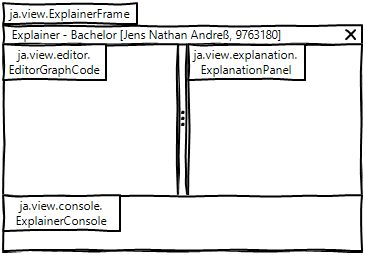
\includegraphics[width=8cm]{chapter/chapter_4/wireframe-impl-overview}
  \caption{Allgemeine Übersicht über das Mockup der Benutzungsschnittstelle.}
  \label{sec4:impl:subsubsec:ui:fig:wireframe-overview}
\end{figure}
\cref{sec4:impl:subsubsec:ui:fig:wireframe-overview} zeigt eine allgemeine Übersicht über das bereits in \cref{sec3:model:par:wireframe:fig:stage-1} vorgestellte Mockup der Benutzungsschnittstelle, erweitert um Zuweisungen der Komponenten mitsamt implementierungsspezifischen Paketnamen.
Die Elemente der in \cref{sec4:impl:subsubsec:ui:fig:wireframe-overview} gezeigten Benutzungsschnittstelle werden in \cref{sec4:impl:par:ui-elements} genauer beschrieben.
Aufbauend auf diesen Elementen wird dann in \cref{sec4:impl:par:ui-interaction} die Interaktion zwischen diesen Elementen beschrieben.
Auf diese Weise entspricht der Ablauf dieses Abschnitts dem Ablauf der Modellierung der Benutzungsschnittstelle.

\subsubsection{Elemente der Benutzeroberfläche}
\label{sec4:impl:par:ui-elements}
% Spezifizierung geschieht dann, ähnlich wie bei der Modellierung in den heruntergebrochenen Benutzungsschnittstellen
% Dem Ablauf der Modellierung folgen und Implementierungen darstellen und untersuchen
% Wichtig hierbei ist keine Logik, sondern erst nur Struktur und notwendige Subkomponenten und Eigenschaften der jeweiligen Schnittstelle...

% Wenn auf Komponente referenziert wird, Essenz der Modellierung rekapitulieren und referenzieren...
% Erst auf die Grundbereiche EditorGraphCode, ExplainerPanel und ExplainerConsole eingehen
% Sinnvoll mit ExplainerConsole zu beginnen?
% Auf jeden Fall erst die Grundbereiche behandeln bevor mit den spezifischeren Komponenten begonnen wird.
% Dann linke Komponente genauer, dann rechte Komponente genauer.


% Komponente ExplainerFrame vorstellen. (Startpunkt bzw. Fundament der Benutzungsschnittstelle ist ExplainerFrame)
% Was ist die Aufgabe des ExplainerFrames? Durch welche Klasse wird diese Komponenten repräsentiert?
% Listing zeigen. (Überlegen was in diesem Listing gezeigt werden soll...?) -> Nur Grundeigenschaften, keine Logik. Kleineres durch Beschreibungen ersetzen..
% Listing erklären...

% ExplainerFrame, kann wie nach der Modellierung, in 3 Teilbereiche aufgeteilt werden (CircleItems) Name Paketname:
% 1) EditorGraphCode (...), 2) ExplainerPanel (...), 3) ExplainerConsole (...)

% Kurze kurze Rekapitulation der Aufgaben dieser Teilbereiche?
% Oder sofort übergehen zu den Listings und danach diese erklären?
% -> Für die jeweiligen Grundbereiche Listings anlegen
% Jedes Listing erklären
% Aber der Reihenfolge der Listings nach
% Bei jedem Grundbereich dann in die Tiefe gehen und wenn alles abgearbeitet ist, dann zum nächsten Grundbereich übergehen

Das Fundament der Benutzungsschnittstelle ist das \textit{ExplainerFrame}, welches durch die Klasse \textit{ja.view.ExplainerFrame} umgesetzt wird.
\cref{sec4:impl:par:ui-elements:lst:explainer-frame} zeigt die wichtigsten Aspekte der Implementierung dieser Klasse.

\lstinputlisting[style=java-code, caption={ExplainerFrame-Klasse}, label={sec4:impl:par:ui-elements:lst:explainer-frame}]{chapter/chapter_4/java/ExplainerFrame.java}

% Erklärung des Listings von ExplainerFrame
Nach der Modellierung enthält dieses Fundament drei Grundbereiche mit folgender Nummerierung (siehe \cref{sec3:model:par:wireframe:fig:stage-1}): \circitem{1} EditorGraphCode, \circitem{2} ExplainerPanel und \circitem{3} ExplainerConsole.
Diese Grundbereiche werden in \cref{sec4:impl:par:ui-elements:lst:explainer-frame} durch die privaten Variablen \textit{editorGraphCode}, \textit{explanationPanel} und \textit{explainerConsole} dargestellt.
Beim Erzeugen der Klasse \textit{ExplainerFrame} wird zuerst durch die Methode \textit{initFrame()} das Frame initialisiert und konfiguriert.
Dies umfasst die Dimension des Frames, die Position, sowie den Titel.
Darauffolgend werden dann durch die Methode \textit{initComponents()} die Komponenten, welches auch die Grundbereiche umfassen, initialisiert, konfiguriert und dem Frame hinzugefügt.
Dies umfasst besonders die notwendigen Schritte zum Hinzufügen und Layouten (z.Dt. Auslegen) der Grundbereiche im \textit{ExplainerFrame}.
Im weiteren Verlauf wird zuerst der Grundbereich \textit{EditorGraphCode}, welcher die linke Arbeitsfläche darstellt, dann der Grundbereich \textit{ExplanationPanel}, welcher die rechte Arbeitsfläche darstellt und schlussendlich der Grundbereich \textit{ExplainerConsole}, welcher die Konsole darstellt, behandelt.
Jeder dieser Grundbereiche wird mitsamt seiner enthaltenen Komponenten ausführlich behandelt, bevor mit dem nächsten Grundbereich fortgefahren wird.

\begin{figure}[!ht]
  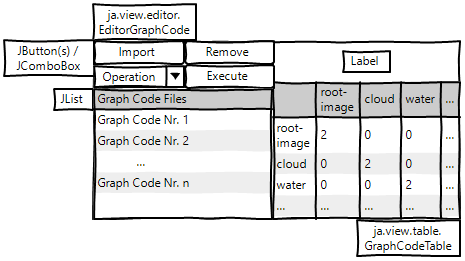
\includegraphics[width=10cm]{chapter/chapter_4/wireframe-impl-left}
  \caption{Grundbereich \textit{EditorGraphCode}.}
  \label{sec4:impl:subsubsec:ui:fig:wireframe-editor-graph-code}
\end{figure}

\cref{sec4:impl:subsubsec:ui:fig:wireframe-editor-graph-code} zeigt den Grundbereich \textit{EditorGraphCode}, umgesetzt durch die Klasse \textit{ja.view.editor.EditorGraphCode}, in welchem Benutzer durch geeignete Interaktionsmöglichkeiten die Bearbeitung von Graph Code Dateien durchführen können.
%Dieser Grundbereich wird durch die Klasse \textit{ja.view.editor.EditorGraphCode} umgesetzt.
\cref{sec4:impl:par:ui-elements:lst:editor-graph-code-p1,sec4:impl:par:ui-elements:lst:editor-graph-code-p2,sec4:impl:par:ui-elements:lst:editor-graph-code-p3,sec4:impl:par:ui-elements:lst:editor-graph-code-p4} zeigen im Folgenden die wichtigsten Aspekte der Implementierung dieser Klasse.

\lstinputlisting[style=java-code, caption={EditorGraphCode-Klasse}, label={sec4:impl:par:ui-elements:lst:editor-graph-code-p1}]{chapter/chapter_4/java/egc/EditorGraphCode-P1.java}

Der Modellierung nach ist diese Arbeitsfläche in zwei nebeneinanderliegende Arbeitsflächen aufgeteilt, die in \cref{sec4:impl:par:ui-elements:lst:editor-graph-code-p1} durch die Variablen \textit{leftPart} und \textit{rightPart} dargestellt werden.
Auch diese Arbeitsflächen bestehen wiederum aus mehreren Komponenten.
Die linke Arbeitsfläche umfasst eine Schnittstelle zum Auswählen und Ausführen von Aktionen (siehe \cref{sec3:model:par:wireframe:fig:stage-2+3} \circitem{4}), dargestellt durch die Variable \textit{operationsPanel} und eine Liste an Graph Code Dateien (siehe \cref{sec3:model:par:wireframe:fig:stage-2+3} \circitem{5}), dargestellt durch die Variable \textit{graphCodeList}.
Die rechte Arbeitsfläche hingegen umfasst im Wesentlichen eine Tabelle zur Visualisierung eines ausgewählten Graph Codes (siehe \cref{sec3:model:par:wireframe:fig:stage-2+3} \circitem{6}), dargestellt durch die Variable \textit{graphCodeTable}, sowie ein Label zum Darstellen des Namens der entsprechenden Graph Code Datei über dieser Tabelle, dargestellt durch die Variable \textit{graphCodeName}.

Im Folgenden wird in \cref{sec4:impl:par:ui-elements:lst:editor-graph-code-p2}, dem zweiten Teil der EditorGraphCode-Klasse, die Schnittstelle \circitem{4} zum Auswählen und Ausführen von Aktionen genauer spezifiziert und im weiteren Verlauf erklärt.

\lstinputlisting[style=java-code, caption={EditorGraphCode-Klasse (Zweiter Teil)}, label={sec4:impl:par:ui-elements:lst:editor-graph-code-p2}, firstnumber=29]{chapter/chapter_4/java/egc/EditorGraphCode-P2.java}

% Erst Zusammenbau der Komponenten erklären (dabei Anwendungsfälle referenzieren)

% Dann später Interaktionen ansprechen und referenzieren

% Am Ende ein Beispiel wie das aussieht?

% Anwendungsfälle referenzieren...
% Dann Mechanismen ansprechen und überleiten zur Interaktion und diese ansprechen bzw. auf entsprechende Klassen verweisen...
% Dann am Ende ein Beispiel... Wie sieht das aus?
Die Schnittstelle zum Auswählen und Ausführen von Aktionen, dargestellt durch \textit{operationsPanel}, besitzt vier Elemente.
Diese Elemente sind JButtons bzw. Knöpfe und eine JComboBox bzw. ein Button mit einer aus- und einklappbaren Auswahlliste und werden im Folgenden aufgezählt:
\begin{itemize}
  \item Knopf \enquote{Import Graph Code(s)}.
  Dieser Knopf ist mit dem Anwendungsfall \hyperref[sec3:model:uc-1.1]{UC-1.1} \enquote{Graph Code(s) importieren} verbunden und wird im Quellcode als Variable \textit{openGraphCodeChooserButton} eingeführt.
  Weiterhin wird die Interaktion durch ein Steuerelement \textit{ImportGraphCodesController}, welches in einem Mechanismus (siehe \cref{sec3:model:par:mechanism-use-cases:fig:mech-uc-1.1}) identifiziert werden konnte, gesteuert.
  Das an diesem Anwendungsfall beteiligte Steuerelement \textit{ImportGraphCodesController} wird in ... genauer behandelt.
  \item Knopf \enquote{Remove selected Graph Code(s)}.
  Dieser Knopf ist mit dem Anwendungsfall \hyperref[sec3:model:uc-1.2]{UC-1.2} \enquote{Graph Code(s) entfernen} verbunden und wird im Quellcode als Variable \textit{removeSelectedButton} eingeführt.
  Weiterhin wird die Interaktion durch ein Steuerelement \textit{RemoveSelectedGraphCodesController}, welches in einem Mechanismus (siehe \cref{sec3:model:par:mechanism-use-cases:fig:mech-uc-1.2}) identifiziert werden konnte, gesteuert.
  Das an diesem Anwendungsfall beteiligte Steuerelement \textit{RemoveSelectedGraphCodesController} wird in ... genauer behandelt.
  \item Aus- und einklappbare Auswahlliste.
  Diese Auswahlliste ist mit dem Anwendungsfall \hyperref[sec3:model:uc-1.4]{UC-1.4} \enquote{Operation auswählen} verbunden und wird im Quellcode als Variable \textit{calculationComboBox} eingeführt.
  Die Interaktion mit diesem Element wird durch das Steuerelement \textit{GraphCodeCalculationController}, welches in einem Mechanismus (siehe \cref{sec3:model:par:mechanism-use-cases:fig:mech-uc-1.5}) identifiziert werden konnte, gesteuert.
  Das an diesem Anwendungsfall beteiligte Steuerelement \textit{GraphCodeCalculationController} wird in ... genauer behandelt.
  \item Knopf \enquote{Execute}.
  Dieser Knopf ist mit dem Anwendungsfall \hyperref[sec3:model:uc-1.5]{UC-1.5} verbunden und wird im Quellcode als Variable \textit{calculationOperationButton} eingeführt.
  Weiterhin wird die Interaktion ebenfalls durch das Steuerelement \textit{GraphCodeCalculationController} gesteuert.
\end{itemize}
Schlussendlich ist in \cref{sec4:impl:par:ui-elements:lst:editor-graph-code-p2} zu sehen, wie die Elemente der Schnittstelle hinzugefügt werden.
Die aus der Implementierung resultierende Schnittstelle zum Auswählen und Ausführen von Aktionen kann in \cref{sec4:impl:par:ui-elements:fig:wireframe-ui-4} eingesehen werden.

\begin{figure}[!ht]
  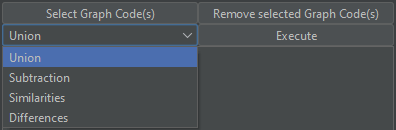
\includegraphics[width=9cm]{chapter/chapter_4/wireframe-impl-ui-4}
  \caption{Aus der Implementierung resultierende Schnittstelle zum Auswählen und Ausführen von Aktionen.}
  \label{sec4:impl:par:ui-elements:fig:wireframe-ui-4}
\end{figure}

Im Folgenden wird in \cref{sec4:impl:par:ui-elements:lst:editor-graph-code-p3}, dem dritten Teil der EditorGraphCode-Klasse, die Schnittstelle \circitem{5} bzw. Liste von Graph Codes genauer spezifiziert und im weiteren Verlauf erklärt.

\lstinputlisting[style=java-code, caption={EditorGraphCode-Klasse (Dritter Teil)}, label={sec4:impl:par:ui-elements:lst:editor-graph-code-p3}, firstnumber=52]{chapter/chapter_4/java/egc/EditorGraphCode-P3.java}

% Zuerst werden Eigenschaften konfiguriert...
% Dann sollte auf den Anwendungsfall und den Mechanismus verwiesen werden und die darin identifizierten Komponenten
% Daher ist es zwischen diesem und dem nächsten listing wohl auch wichtig noch auf die Grundkomponente der Liste einzugehen (in Bezug auf den Mechanismus)... (GraphCodeListElement)...
% "Des Weiteren konnte im Mechanismus die Komponente GraphCodeListElement identifiziert werden, die ein Element bzw. Eintrag in der Liste dargestellt"...

% Dann noch ein echtes Beispiel für diese Liste mit Inhalt (Graph Codes)

Zuerst werden Eigenschaften der Liste konfiguriert.
Eine dieser Eigenschaften ist z.B. der Auswahlmodus \textit{MULTIPLE\_INTERVAL\_SELECTION}, um ein mehrfache Auswahl in der Liste zu ermöglichen.

Die Liste ist mit dem Anwendungsfall \hyperref[sec3:model:uc-1.3]{UC-1.3} \enquote{Graph Code(s) auswählen} verbunden.
In Bezug auf den Anwendungsfall wird die Interaktion mit der Liste durch das Steuerelement \textit{GraphCodeSelectionListener} gesteuert, welches in einem Mechanismus (siehe \cref{sec3:model:par:mechanism-use-cases:fig:mech-uc-1.3}) identifiziert werden konnte.
Das Steuerelement \textit{GraphCodeSelectionListener} wird in ... genauer behandelt.
Zusätzlich besitzt die Liste weitere Steuerelemente, die ebenfalls in ... genauer behandelt werden.
Des Weiteren konnte in diesem Mechanismus, wie bereits auch schon in den vorherigen Mechanismen, die Komponente \textit{GraphCodeListElement} identifiziert werden.
Diese Komponenten ist in Bezug auf die Liste von besonderer Bedeutung, da diese ein Element bzw. Eintrag in der Liste darstellt.
Der Quellcode für diese Komponente kann in \cref{sec4:impl:par:ui-elements:lst:gcle} eingesehen werden.

\lstinputlisting[style=java-code, caption={GraphCodeListElement-Klasse}, label={sec4:impl:par:ui-elements:lst:gcle}, firstnumber=1]{chapter/chapter_4/java/gcle/GraphCodeListElement.java}

\cref{sec4:impl:par:ui-elements:fig:wireframe-ui-5} zeigt ein Beispiel für die aus der Implementierung resultierende Liste mitsamt beispielhaften Einträgen für Graph Codes.

\begin{figure}[!ht]
  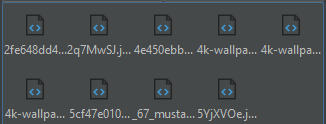
\includegraphics[width=9cm]{chapter/chapter_4/wireframe-impl-ui-5}
  \caption{Aus der Implementierung resultierende Liste mit beispielhaften Einträgen für Graph Codes.}
  \label{sec4:impl:par:ui-elements:fig:wireframe-ui-5}
\end{figure}

Schlussendlich wird in \cref{sec4:impl:par:ui-elements:lst:gct} die letzte Schnittstelle \circitem{6} \textit{GraphCodeTable} des Grundbereichs \textit{EditorGraphCode} behandelt und im weiteren Verlauf erklärt.

\lstinputlisting[style=java-code, caption={GraphCodeTable-Klasse}, label={sec4:impl:par:ui-elements:lst:gct}, firstnumber=1]{chapter/chapter_4/java/gct/GraphCodeTable.java}

Die Schnittstelle \textit{GraphCodeTable} besitzt zwei Elemente: Eine Tabelle zur Darstellung eines ausgewählten Graph Codes, umgesetzt durch ein \textit{JTable} und ein Platzhalter, zum Signalisieren, dass zu diesem Zeitpunkt noch kein Graph Code ausgewählt ist / wurde.
Die Tabelle wird in einem \textit{JScrollPane} eingebettet, um auch größere Tabellen darstellen zu können.
Des Weiteren ist ein wichtiger Teil dieser Klasse ein Datenmodell für die Tabelle, dargestellt durch die Komponente \textit{GraphCodeTableModel}.
Dieses Datenmodell wird der Tabelle zugewiesen und hat zur Aufgabe, die Informationen in einem Graph Code auf die Zeilen und Spalten der Tabelle abzubilden, sodass diese in Tabellenform dargestellt werden können.
Die wichtigste Methode dieser Klasse ist die Methode \textit{setGraphCode}.
Diese Methode nimmt als Parameter einen ausgewählten Graph Code.
Anhand dieses Graph Codes werden Veränderungen an der Schnittstelle, sowie dem Datenmodell vorgenommen.
Sofern kein Graph Code ausgewählt ist, wird ein Platzhalter angezeigt.
Andernfalls wird dem Datenmodell der Graph Code zur Verarbeitung zugewiesen.

\cref{sec4:impl:par:ui-elements:fig:wireframe-ui-6} zeigt ein Beispiel für die aus der Implementierung resultierende Tabelle zur Darstellung eines ausgewählten Graph Codes.

\begin{figure}[!ht]
  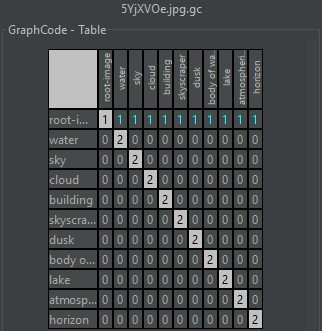
\includegraphics[width=8cm, keepaspectratio]{chapter/chapter_4/wireframe-impl-ui-6}
  \caption{Aus der Implementierung resultierende Tabelle zur Darstellung eines ausgewählten Graph Codes.}
  \label{sec4:impl:par:ui-elements:fig:wireframe-ui-6}
\end{figure}

Im Folgenden wird in \cref{sec4:impl:par:ui-elements:lst:editor-graph-code-p4}, der vierte und letzte Teil der EditorGraphCode-Klasse, genauer spezifiziert und im weiteren Verlauf erklärt.

\lstinputlisting[style=java-code, caption={EditorGraphCode-Klasse (Letzter Teil)}, label={sec4:impl:par:ui-elements:lst:editor-graph-code-p4}, firstnumber=58]{chapter/chapter_4/java/egc/EditorGraphCode-P4.java}

\cref{sec4:impl:par:ui-elements:lst:editor-graph-code-p4} zeigt das abschließende Zusammenfügen der Schnittstellen \circitem{4}, \circitem{5} und \circitem{6}.
Zusammengefügt ergeben diese Schnittstellen den Grundbereich \textit{EditorGraphCode}.
Damit ist der Grundbereich \circitem{1}, \textit{EditorGraphCode}, abgeschlossen.
\cref{sec4:impl:par:ui-elements:fig:wireframe-ui-left-complete} zeigt abschließend die vollständige Benutzeroberfläche des aus der Implementierung resultierenden Grundbereichs \textit{EditorGraphCode} mitsamt Beispielen.

\begin{figure}[!ht]
  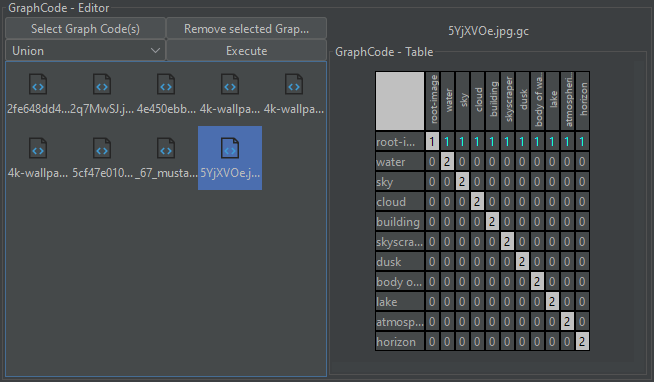
\includegraphics[width=\textwidth]{chapter/chapter_4/wireframe-impl-ui-left-complete}
  \caption{Vollständige Oberfläche des aus der Implementierung resultierenden Grundbereichs \textit{EditorGraphCode}.}
  \label{sec4:impl:par:ui-elements:fig:wireframe-ui-left-complete}
\end{figure}

% Überleitung zum nächsten Grundbereich ExplanationPanel...
% Dann mit Grundbereich ExplanationPanel fortfahren...

\begin{figure}[!ht]
  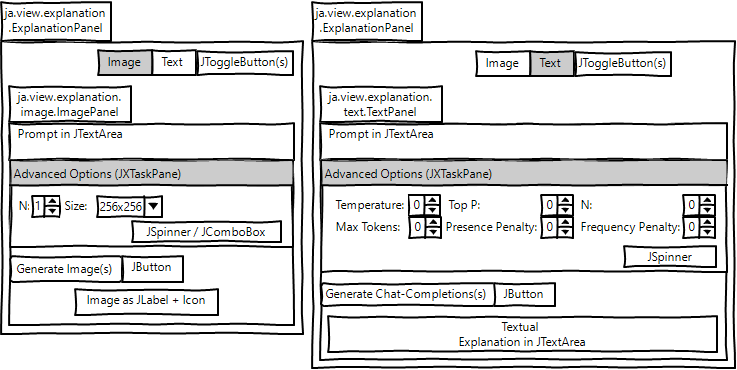
\includegraphics[width=\textwidth]{chapter/chapter_4/wireframe-impl-right}
  \caption{Grundbereich \textit{ExplanationPanel} zur Generierung von visuellen Erklärungen (links) und textuellen Erklärungen (rechts).}
  \label{sec4:impl:subsubsec:ui:fig:wireframe-explanation-panel}
\end{figure}

\cref{sec4:impl:subsubsec:ui:fig:wireframe-explanation-panel} zeigt den Grundbereich \textit{ExplanationPanel}, umgesetzt durch die Klasse \textit{ja.view.explanation.ExplanationPanel}, in welchem Benutzer durch geeignete Interaktionsmöglichkeiten die Generierung von visuellen und textuellen Erklärungen zu Graph Codes durchführen können.
Hierzu besitzt der Grundbereich \textit{ExplanationPanel} eine Fläche bzw. einen Container, in der Komponenten miteinander ausgewechselt werden können.
Genauer wird zwischen zwei Komponenten gewechselt: \textit{ImagePanel} und \textit{TextPanel}.

\lstinputlisting[style=java-code, caption={ExplanationPanel-Klasse}, label={sec4:impl:par:ui-elements:lst:explanation-panel}, firstnumber=1]{chapter/chapter_4/java/exp/ExplanationPanel.java}

\lstinputlisting[style=java-code, caption={ImagePanel-Klasse}, label={sec4:impl:par:ui-elements:lst:image-panel}, firstnumber=1]{chapter/chapter_4/java/exp/img/ImagePanel.java}

\lstinputlisting[style=java-code, caption={TextPanel-Klasse}, label={sec4:impl:par:ui-elements:lst:text-panel}, firstnumber=1]{chapter/chapter_4/java/exp/text/TextPanel.java}

\FloatBarrier

% Bezug zum Forschungsziel anführen.

\subsubsection{Interaktion mit der Benutzeroberfläche}
\label{sec4:impl:par:ui-interaction}
% Hier dann die Komponenten zur Kontrolle der Interaktion vorstellen und dann anhand der Eigenschaften der Oberflächen Logik einfügen und beschreiben. (Nur Logik bezüglich der Interaktion)
% logik bezüglich der Verarbeitung bleibt noch offen und wird dann in FZ 2.3/I behandelt. (somit darauf verweisen)

% Auf Anwendungsfälle, Mechanismen und Sequenzdiagramme eingehen...

\clearpage
